% Faithful initial reconstruction of Annex E from source PDF pages 361--370
% (standard pages 347--356).

\clearpage

% --- Standard page 347 / source PDF page 361 ---
\begin{annexstdpage}
    \stdannexheading{E}{informative}{Rationale}

    \stdannexsection{E.1}{Overview}

    This annex contains additional information that might be useful to explain various aspects of HLA and is not a complete rationale of the HLA. Nothing in this clause is required in an HLA implementation.

    This annex is organized to match the organization of the main body of this specification, and the subclause numbers in this annex correspond to the subclause numbers of the main body. Note, however, that not all subclauses in the main body have corresponding subclauses in this annex. In other words, text is present in this annex only if additional comments were deemed helpful to understanding the corresponding subclauses in the main body.

    \stdannexsubsection{E.1.4}{Background}

    Consideration was given to providing several iterating functions; however, there were found to be serious problems documenting and describing the iterating-based semantics of these services. Additionally, there was a problem with every redaction produced. The candidate definitions of how exceptions were handled and recovered from during the ``middle'' of an iteration sequence never satisfied a large enough set of users to be acceptable for retention in the specification. Each of the users wanted the behavior to meet their specific application needs, which in most cases were inconsistent and impossible to meet with a common mechanism. As a result, it seemed to make the most sense not to have any iterating services and to let users produce their own aggregate functionality with the exception response semantics they needed.

    \stdannexsection{E.4}{Federation management}

    \stdannexsubsection{E.4.6}{\textit{Destroy Federation Execution} service}

    Since there can be no joined federates for the destroy service invocation to succeed, there might be a problem if the federation execution has ``zombie'' or otherwise uncooperative joined federates. To aid matters in this situation, a joined federate can be resigned by another joined federate via a MOM interaction.

    \stdannexsubsection{E.4.31}{\textit{Query Federation Restore Status} service}

    One way to employ federation restore status is for a federation manager federate to not invoke the Restore Complete service until all the other joined federates have successfully completed their restore. In this way, a federation manager federate can ``throttle'' the restore process as it monitors the restore status.
\end{annexstdpage}

\clearpage

% --- Standard page 348 / source PDF page 362 ---
\begin{annexstdpage}
    \stdannexsection{E.5}{Declaration management (DM)}

    \stdannexsubsection{E.5.1}{Overview}

    One reason joined federates can subscribe at multiple levels in a class hierarchy is to allow for FOM growth. As a FOM expands, a federate application need not be recoded. It can continue to subscribe at the same levels in the hierarchy while other, ``newer'' federate applications in the federation can subscribe at the new classes.

    Some services in the interface specification contain postconditions that are less precise than one would expect. The postcondition for the \textit{Subscribe Object Class Attributes} service, for example, states only that ``the RTI has been informed of the joined federate's requested subscription.'' It does not say that the joined federate is now subscribed to the specified class attributes, nor is a statement to this effect found in any service postcondition.

    Services with such imprecise postconditions include the following:

    \begin{stddashlist}
        \item \textit{Subscribe Object Class Attributes}
        \item \textit{Subscribe Interaction Class}
        \item \textit{Commit Region Modifications} (old Modify Region)
        \item \textit{Subscribe Object Class Attributes With Regions}
        \item \textit{Subscribe Interaction Class With Regions}
    \end{stddashlist}

    These services have imprecise postconditions, similar to the postcondition quoted above, because the interface specification allows RTI implementations to decide when to determine whether a message sent by one federate should be received by another federate. One possibility is to broadcast all sent messages and perform filtering at each receiving federate. A more efficient possibility is to perform filtering when the message is sent (in other words, the message is sent only to interested federates) and again at each receiving federate (in case the state of the receiver has changed during transmission).

    The problem with allowing the latter alternative is that should the receiver add to its subscriptions, that addition cannot be considered to have fully taken effect until the RTI can ensure that messages sent by any federate will take the added subscriptions into account, thus the imprecise postconditions. Subscription additions take effect locally immediately, but there will be some delay before the additions take effect throughout the federation execution. An RTI implementation must ensure that these changes take effect throughout the federation execution as soon as possible, but it will not delay the return of these service invocations until it can guarantee the subscription additions are complete.

    Since federates can come and go and can add subscriptions at any wall-clock time, the only way the RTI could meet a postcondition asserting that the federate is now subscribed to the specified attributes would be to synchronize the whole federation execution so that it could make that guarantee. This is one of the places in the specification where the desire was to permit more federate asynchronous behavior. This places more responsibility on the federates to ensure that they know what they are doing and make their subscriptions in sufficient wall-clock time for them to have the desired effect in their federation execution.

    \stdannexsubsection{E.5.1.2}{Definitions and constraints for object classes and class attributes}

    Item (o) in 5.1.2 is a very complex sentence, and it has been suggested that it may be difficult for the reader to parse and understand. This text is an attempt to explain what it means by example.
\end{annexstdpage}

\clearpage

% --- Standard page 349 / source PDF page 363 ---
\begin{annexstdpage}
    Consider Figure E.1, the object class inheritance tree.

    \begin{center}
        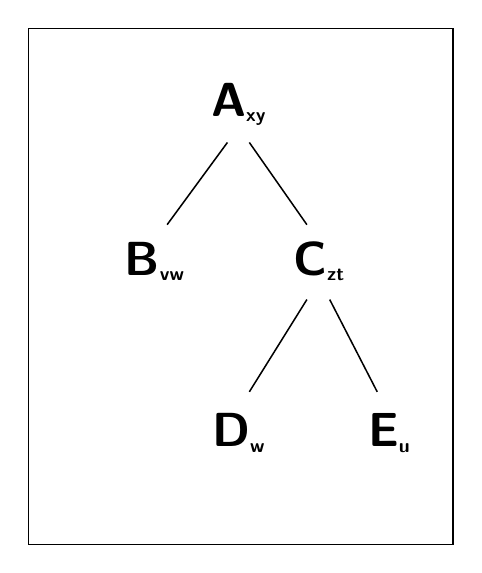
\begin{tikzpicture}[x=1.16cm,y=1.16cm]
            \draw[line width=.45pt] (0,0) rectangle (4.65,5.65);
            \node[font=\sffamily\bfseries\fontsize{17}{18}\selectfont] (A) at (2.30,4.82) {A\raisebox{-.25ex}{\scriptsize xy}};
            \node[font=\sffamily\bfseries\fontsize{17}{18}\selectfont] (B) at (1.38,3.10) {B\raisebox{-.25ex}{\scriptsize vw}};
            \node[font=\sffamily\bfseries\fontsize{17}{18}\selectfont] (C) at (3.18,3.10) {C\raisebox{-.25ex}{\scriptsize zt}};
            \node[font=\sffamily\bfseries\fontsize{17}{18}\selectfont] (D) at (2.30,1.22) {D\raisebox{-.25ex}{\scriptsize w}};
            \node[font=\sffamily\bfseries\fontsize{17}{18}\selectfont] (E) at (3.95,1.22) {E\raisebox{-.25ex}{\scriptsize u}};
            \draw[line width=.55pt] (2.18,4.40) -- (1.52,3.50);
            \draw[line width=.55pt] (2.42,4.40) -- (3.05,3.50);
            \draw[line width=.55pt] (3.05,2.68) -- (2.42,1.67);
            \draw[line width=.55pt] (3.30,2.68) -- (3.82,1.67);
        \end{tikzpicture}

        \vspace{2pt}
        {\sffamily\bfseries\fontsize{9.0}{10.4}\selectfont Figure E.1---Example object class inheritance tree}
    \end{center}

    The following notation is used in this example:

    \begin{stddashlist}
        \item \textbf{Subscribe [C(z)]} denotes the invocation of the \textit{Subscribe Object Class Attributes} service to subscribe to object class C and class attribute z.
        \item \textbf{Publish [E(x, u)]} denotes the invocation of the \textit{Publish Object Class Attributes} service to publish object class E and class attributes x and u.
        \item \textbf{Register (E, e1)} denotes the invocation of the \textit{Register Object Instance} service to register an object instance of class E that will be denoted e1.
        \item \textbf{e1(x)} denotes instance attribute x of object instance e1.
    \end{stddashlist}

    Suppose federate \textit{F} invokes

    \begin{stddashlist}
        \item Subscribe [C(z)]
        \item Subscribe [A(x,y)]
    \end{stddashlist}

    Suppose federate \textit{H} invokes

    \begin{stddashlist}
        \item Subscribe [C(x,z)]
        \item Subscribe [A(y)]
    \end{stddashlist}

    Suppose federate \textit{G} invokes

    \begin{stddashlist}
        \item Publish [C(z,t)]
        \item Publish [E(x,y,u)]
        \item Register (E, e1)
    \end{stddashlist}

    Then

    \begin{stddashlist}
        \item \textbf{Ownership:} Federate \textit{G} now owns e1(x), e1(y), and e1(u). Even though federate \textit{G} was publishing class attributes z and t when it registered e1, federate \textit{G} was not publishing z or t at the registered class of e1 (class E) when it registered e1; therefore, federate \textit{G} does not own e1(z) or e1(t). e1(z) and e1(t) are not owned by any federate.
    \end{stddashlist}
\end{annexstdpage}

\clearpage

% --- Standard page 350 / source PDF page 364 ---
\begin{annexstdpage}
    \begin{stddashlist}
        \item \textbf{Discovery at Federate F:} Federate F will not discover object instance e1. The candidate discovery class of e1 at federate F is class C. But federate F is not subscribed to any class attribute at class C that has a corresponding instance attribute that is part of e1 and that is owned. Therefore, object instance e1 is not known to federate F, and it has no known class at federate F. Federate F is not capable of receiving reflects for updates made to any values of the instance attributes of object instance e1. Even though federate F is subscribed to class attribute x at class A, an update made to instance attribute e1(x) will not be reflected at federate F because e1 is not known to federate F. (For more information on discovery and known classes, see also 6.1.)
        \item \textbf{Discovery at Federate H:} Federate H will discover object instance e1 as a class C object instance. The candidate discovery class of e1 at federate H is class C because federate H is not subscribed to e1's registered class (class E) and class C is the closest superclass of e1's registered class to which federate H is subscribed. Federate H is also subscribed to class attribute x at class C, and class attribute x has a corresponding instance attribute that is part of object instance e1 and that is owned, namely e1(x). Therefore, the known class of e1 at federate H is class C.
        \item \textbf{Reflection:} When federate G updates the value of e1(x), this update will be reflected at Federate H. However, when federate G updates the value of e1(y) or e1(u), these updates will not be reflected at federate H because federate H is not subscribed to class attributes y or u at class C. Notice that even though federate H is subscribed to class attribute y, it will not receive reflects for updates made to the value of e1(y) because federate H is not subscribed to class attribute y at the known class (class C) of e1.
    \end{stddashlist}

    Recall the wording of item (o) of 5.1.2, which says, ``An update to an instance attribute by the federate that owns that instance attribute shall be reflected only by other federates that are subscribed to the instance attribute's corresponding class attribute at the known class of the object instance that contains that instance attribute at the subscribing federate.'' In terms of this example, this wording means the following:

    \begin{quote}
        An update to e1(x) by federate G shall be reflected by federate H because federate H is subscribed to class attribute x at e1's known class at federate H (namely, class C). An update to e1(y) or e1(u) by federate G shall not be reflected by federate H because federate H is not subscribed to class attributes y or u at e1's known class at H (class C).
    \end{quote}

    \stdannexsection{E.6}{Object management}

    \stdannexsubsection{E.6.1}{Overview}

    For examples that further elucidate the concepts of discovery and known class, see E.5.1.2 and E.9.1.5.

    If an instance attribute is in scope for a given joined federate F, there exists at least one other joined federate in the federation execution that is capable of invoking the \textit{Update Attribute Values} service for that instance attribute so that if that joined federate were to invoke the \textit{Update Attribute Values} service for that instance attribute, all of the preconditions for the invocation of the corresponding \textit{Reflect Attribute Values} \rtiinitiated\ service at federate F are satisfied. Therefore, if an instance attribute is in scope for a given joined federate, that joined federate may receive invocations of the \textit{Reflect Attribute Values} \rtiinitiated\ service for that instance attribute. It is also possible, however, for a joined federate to receive invocations of the \textit{Reflect Attribute Values} \rtiinitiated\ service for an instance attribute that is not in scope for that joined federate. All of the conditions that define whether an instance attribute is in scope are also preconditions of the \textit{Reflect Attribute Values} \rtiinitiated\ service, with the exception of the condition that the instance attribute be owned by another joined federate. Because the conditions for determining whether an instance attribute is in scope are more restrictive than the conditions for determining whether an update to that instance attribute should be reflected, it is possible for updates to instance attributes that are not in scope to be reflected.
\end{annexstdpage}

\clearpage

% --- Standard page 351 / source PDF page 365 ---
\begin{annexstdpage}
    As an illustrative example, consider the scenario in which a joined federate that owns a particular instance attribute invokes the \textit{Update Attribute Values} service for that instance attribute using a timestamp argument indicating a federation time far into the future. Then, that joined federate divests ownership of the instance attribute and resigns from the federation execution. No other joined federate acquires ownership of the instance attribute. When the federation time indicated in the timestamp argument of the update arrives, that instance attribute is, by definition, out of scope for all joined federates in the federation execution because it is not owned. Nevertheless, assuming all of the other preconditions for invocation of the \textit{Reflect Attribute Values} \rtiinitiated\ service for that instance attribute are satisfied at a given joined federate, the \textit{Reflect Attribute Values} \rtiinitiated\ service will be invoked at that joined federate. Hence, an instance attribute being in or out of scope for a particular joined federate indicates only whether there is some other joined federate in the federation execution that is capable of generating updates to that instance attribute so that if that joined federate were to invoke the \textit{Update Attribute Values} service for that instance attribute, all of the preconditions for the invocation of the corresponding \textit{Reflect Attribute Values} \rtiinitiated\ service at federate F are satisfied. An instance attribute being in or out of scope for a particular joined federate makes no assertion regarding whether invocations of the \textit{Reflect Attribute Values} \rtiinitiated\ service for that instance attribute may be invoked at that joined federate.

    \stdannexsubsection{E.6.5}{\textit{Reserve Multiple Object Instance Names} service}

    The multiple name reservation services provide a shortcut method for reserving multiple object instance names. Since a centralized or distributed name reservation implementation would require synchronization across the network for each name reservation transaction, this shortcut can reduce the overhead of reserving multiple object names.

    \stdannexsubsection{E.6.14}{\textit{Delete Object Instance} service}

    It should be noted in conjunction with this service that this standard is silent regarding what will happen in the case in which a joined federate attempts to take ownership of an instance attribute of an object instance for which another joined federate has already scheduled a timed deletion. In other words, if a joined federate schedules the deletion of an object instance for a federation time in the future, that object instance may still be discovered by other joined federates, and updates to instance attributes of that object instance may still be received by other joined federates, until their logical times are greater than or equal to the specified federation time of the deletion. If those other joined federates are allowed to take ownership of any of the instance attributes owned by the joined federate that scheduled the delete, then it would be possible for anomalous events to occur within the federation execution, such as a joined federate that owns the HLAprivilegeToDeleteObject instance attribute of an object instance receiving an invocation of the \textit{Remove Object Instance} \rtiinitiated\ service for that object instance. This standard does not specify the RTI's behavior in such circumstances.

    \stdannexsubsection{E.6.19}{\textit{Request Attribute Value Update} service}

    A single \textit{Request Attribute Value Update} service invocation for an object class may generate many \textit{Provide Attribute Value Update} \rtiinitiated\ service invocations at instance attribute-owning joined federates (at least one for each object instance of the class for which the joined federate owns a requested attribute). This situation will generate a nonpredictable ``storm'' of ``interrupts'' and possibly cause the timing behavior of real-time federates to become unpredictable. This might be an unwise thing to do in a real-time federation.

    \stdannexsubsection{E.6.23}{\textit{Request Attribute Transportation Type Change} service}

    Actual implementation of the transportation types are RTI implementation dependent. The names may be declared in FOM/FDD.
\end{annexstdpage}

\clearpage

% --- Standard page 352 / source PDF page 366 ---
\begin{annexstdpage}
    \stdannexsection{E.8}{Time management}

    \stdannexsubsection{E.8.1}{Overview}

    At the federation level, this specification provides a variety of time management services to control the advancement of all joined federates along the HLA time axis. These services allow multiple joined federates with differing internal federation time advancement strategies to interoperate in a meaningful way. While the strategy chosen for advancing federation time is an extremely important consideration in the design of a simulation, the format of how federation time is represented is of equal importance.

    It is very important for all federation members to agree upon a common set of key federation time characteristics that apply across the full federation. In addition to defining certain characteristics of the HLA time axis, it is also important to define the lookahead characteristics of both federates and federations. It is important to recognize that there are semantic differences between the way federation time is represented for the purpose of advancing federation time versus calculating lookahead. When advancing federation time, federation time can be considered to be an absolute value on a federation timeline, and thus federation time comparisons can be drawn to determine if one federation time value is greater than another. Lookahead, in contrast, represents a duration of federation time, which can be added to absolute federation time values but is not generally used for comparison purposes. For this reason, federation time is defined using two abstract datatypes (ADTs), LogicalTime and LogicalTimeInterval.

    Each of the specific language APIs contain ADTs for LogicalTime and LogicalTimeInterval. These ADTs each define a set of interfaces for which implementations must be provided before a federation execution that utilizes time management services can take place. It is the responsibility of the federate/federation developer(s) to furnish concrete implementations of LogicalTime and LogicalTimeInterval interfaces.

    Additionally, each of the language APIs also provide default concrete implementations of these two ADTs based on the float 64 datatype.

    \stdannexsubsection{E.8.1.1}{Messages}

    While this specification states no explicit requirements on the order of delivery of RO messages, an RTI implementation may provide a more predictable order of delivery. A number of factors must be considered by an RTI when determining the order in which RO messages are received, including the following:

    \begin{stddashlist}
        \item Whether a series of messages sent from the same federate are delivered in the same order as the order in which they were sent
        \item Whether series of messages sent by different federates are interleaved
        \item Whether messages received as RO that were sent as RO and that were sent as TSO are interleaved
    \end{stddashlist}

    A federate that assumes a particular ordering of RO messages may not be able to freely choose among RTI implementations.

    A federate may choose to send TSO messages using different transportation types, but if the delivery mechanism is unreliable, there may be circumstances in which the message must be delivered to a receiving, time-constrained federate as RO. Federation time synchronization mechanisms typically rely on reliable message delivery to efficiently advance along the HLA time axis, and messages transmitted unreliably may be delivered with a timestamp that would violate causality for a receiving federate. Under these circumstances, an RTI must deliver the TSO message as RO.
\end{annexstdpage}

\clearpage

% --- Standard page 353 / source PDF page 367 ---
\begin{annexstdpage}
    \stdannexsubsection{E.8.6}{\textit{Time Constrained Enabled} \rtiinitiated\ service}

    This service description says that (if the joined federate is not time-regulating) ``the RTI shall provide the joined federate with the smallest possible logical time that is greater than or equal to the logical time of the joined federate and for which all other constraints necessary to ensure TSO message delivery are satisfied.'' This description is overly complicated.

    When a joined federate invokes the \textit{Enable Time Constrained} service, there is no case in which the joined federate's logical time needs to be advanced. The value of the current logical time argument of the \textit{Time Constrained Enabled} \rtiinitiated\ service will always be the current logical time of the joined federate when it invoked the \textit{Enable Time Constrained} service.

    If the joined federate's current logical time is less than or equal to its GALT when it invokes the \textit{Enable Time Constrained} service, then the \textit{Time Constrained Enabled} \rtiinitiated\ service may be invoked immediately at the joined federate. If the joined federate's current logical time is greater than its GALT when it invokes the \textit{Enable Time Constrained} service, then the \textit{Time Constrained Enabled} \rtiinitiated\ service cannot be invoked until the joined federate's GALT advances beyond its logical time. In either case, however, when the \textit{Time Constrained Enabled} \rtiinitiated\ service is invoked at the joined federate, the value of the current logical time argument of the \textit{Time Constrained Enabled} \rtiinitiated\ service will be the value of the joined federate's current logical time when the joined federate invoked the \textit{Enable Time Constrained} service.

    \stdannexsubsection{E.8.12}{\textit{Flush Queue Request} service}

    The \textit{Flush Queue Request} service introductory text says,

    \begin{quote}
        The RTI shall advance the joined federate's logical time to the smallest of the following:
        \begin{stddashlist}
            \item The specified logical time
            \item The joined federate's GALT value
            \item The smallest timestamp of all TSO messages delivered by the RTI in response to this invocation of the \textit{Flush Queue Request} service
        \end{stddashlist}
    \end{quote}

    The third item in the list above is a change from the 1.3 version to the HLA specification, and the purpose of adding it is to allow federates to generate new events with ``small'' timestamps in response to events it received as a result of the \textit{Flush Queue Request}. For example, consider the following scenario:

    \begin{quote}
        A federate makes a \textit{Flush Queue Request} service invocation to federation time 100.

        The federate receives a message with timestamp 95.

        The federate gets a grant to federation time T.

        Without the third condition above, the federate could get a grant up to federation time 100 (i.e., T=100). However, the federate may want to send a new event, e.g., \textit{Update Attribute Values}, in response to the event with timestamp 95. This new event might have, for example, a timestamp of 96. This is a perfectly reasonable thing to do, but would cause an exception if the federate had already been advanced to federation time 100.

        To address this situation, the third condition will ensure that the grant will only be to federation time 95 (or less).
    \end{quote}
\end{annexstdpage}

\clearpage

% --- Standard page 354 / source PDF page 368 ---
\begin{annexstdpage}
    \stdannexsubsection{E.8.22}{\textit{Request Retraction} \rtiinitiated\ service}

    Federates should be aware that, according to this service description, they may receive a \textit{Request Retraction} \rtiinitiated\ callback for a message that has not been delivered to them. In this case, federates should ignore the \textit{Request Retraction} \rtiinitiated\ callback.

    \stdannexsection{E.9}{Data distribution management (DDM)}

    \stdannexsubsection{E.9.1.5}{Reinterpretation of selected declaration management services}

    See E.5.1.2 for an explanation of item (o) of 5.1.2 when regions are not being used for update of an instance attribute or used for subscription of a class attribute. The following example is intended to explain item (o) of 9.1.1 when regions are being used for update of an instance attribute or used for subscription of a class attribute.

    Consider the same object class inheritance tree as pictured in Figure E.1. The following notation is used in this example in addition to that which was introduced in E.5.1.2:

    \begin{stddashlist}
        \item \textbf{Subscribe\_w\_Reg [C,R1,(x,z)]} denotes the invocation of the \textit{Subscribe Object Class Attributes With Regions} service to subscribe to object class C and class attributes x and z and to use region R1 for subscription of class attributes x and z.
        \item \textbf{Register\_w\_Reg [E, (R1,x), (R2,y),e1]} denotes the invocation of the \textit{Register Object Instance With Regions} service to register an object instance of class E that will be denoted e1 and to use region R1 for update of instance attribute e1(x) and region R1 for update of instance attribute e1(y).
    \end{stddashlist}

    Suppose that all class attributes in this example have the same set of available dimensions.

    Suppose regions R1, R2, and R3 have been created, and each of these regions contains all of the available dimensions of the class attributes in this example.

    Suppose that

    \begin{stddashlist}
        \item Regions R1 and R2 overlap
        \item Regions R1 and R3 do not overlap
    \end{stddashlist}

    Suppose federate H invokes

    \begin{stddashlist}
        \item Subscribe\_w\_Reg [C,R1,(x,z,t)]
        \item Subscribe\_w\_Reg [A,R1,(y)]
    \end{stddashlist}

    Suppose federate G invokes

    \begin{stddashlist}
        \item Publish [E(x,y,z,t,u)]
        \item Register\_w\_Reg [E, (R2,x),(R2,y),(R3,z),e1]
    \end{stddashlist}

    Then

    \begin{stddashlist}
        \item \textbf{Ownership:} Federate G now owns e1(x), e1(y), e1(z), e1(t), and e1(u). Region R2 is used for update of e1(x) and e1(y) by federate G; region R3 is used for update of e1(z) by federate G; and the default region is used for update of e1(t) and e1(u) by federate G. By definition, R1, R2, and R3 all overlap with the region used for update of e1(t) and e1(u).
    \end{stddashlist}
\end{annexstdpage}

\clearpage

% --- Standard page 355 / source PDF page 369 ---
\begin{annexstdpage}
    \begin{stddashlist}
        \item \textbf{Discovery at federate H:} Federate H will discover object instance e1 as a class C object instance. The candidate discovery class of e1 at federate H is class C because federate H is not subscribed to e1's registered class (class E) and class C is the closest superclass of e1's registered class to which federate H is subscribed. Federate H is also subscribed to class attribute x at class C with region R1, and class attribute x has a corresponding instance attribute that is part of object instance e1 and that is owned (namely e1(x)). Region R2 is used for update of e1(x) by its owning federate (federate G), and regions R1 and R2 overlap. Therefore, the known class of e1 at federate H is class C.
        \item \textbf{Reflection:} When federate G updates the value of e1(x) or e1(t), these updates shall be reflected at federate H. Updates to e1(x) and e1(t) will be reflected at federate H because federate H is subscribed to class attributes x and t at e1's known class (class C), and the region that is used for subscription of x and t by federate H (region R1) overlaps the region that is used for updates of e1(x) and e1(t) by owning federate G (namely, region R2 in the case of e1(x) and the default region of routing space R in the case of e1(t)). However, when federate G updates the value of e1(y), e1(z), or e1(u), these updates will not be reflected at federate H. Updates to e1(y) and e1(u) will not be reflected at federate H because federate H is not subscribed to class attribute y at object instance e1's known class (class C) and class attribute u is not even available for subscription at object instance e1's known class (class C). Federate H is subscribed with region to class attribute z at e1's known class, but updates to e1(z) will not be reflected at federate H because federate H is using region R1 for subscription of class attribute z, federate G is using region R3 for update of instance attribute e1(z), and these two regions (R1 and R3) do not overlap.
    \end{stddashlist}

    \stdannexsubsection{E.9.13}{\textit{Request Attribute Value Update With Regions} service}

    Unlike the corresponding object management service (Request Attribute Value Update), this service does not allow an object instance to be used as an argument; only an object class can be used. If an update for attributes of a specific object instance is needed, the object management service should be used. As a request that takes an object instance is already quite specific, additional DDM filtering based on regions is not needed for such cases.

    A single \textit{Request Attribute Value Update With Regions} service invocation for an object class may generate many \textit{Provide Attribute Value Update} \rtiinitiated\ service invocations at instance attribute-owning joined federates (at least one for each object instance of the class for which the joined federate owns a requested attribute). This situation will generate a nonpredictable ``storm'' of ``interrupts'' and possibly cause the timing behavior of real-time federates to become unpredictable. This might be an unwise thing to do in a real-time federation.

    \stdannexsection{E.11}{Management object model (MOM)}

    The defined MOM functionality is necessary for successful federation execution operation and can be provided only by the RTI. The MOM definition needs to be standardized by defining it in this specification.

    Remotely changing joined federate states (e.g., publication, transportation types, time management) as provided by the MOM can be error prone. However, these sorts of actions are needed in federations to recover from catastrophic error conditions. They should be used with extreme caution.

    Additionally, there are ways a federate can ascertain that MOM has done something ``on its behalf.'' The ``target'' federate can subscribe to ModifyAttributeState and all Manager.Federate.Service interactions and inspect them to determine if other federates are attempting to change its owned attribute state or invoke HLA services on its behalf. The only issue is that the RTI may react to the MOM interaction before the affected federate receives the particular notifying interaction.
\end{annexstdpage}

\clearpage

% --- Standard page 356 / source PDF page 370 ---
\begin{annexstdpage}
    \stdannexsubsection{E.11.6}{MOM OMT tables}

    In Table 4 (in 11.6), the HLAObjectRoot object is present as a class in which to house the \textbf{HLAprivilegeToDeleteObject} object class attribute. Additionally, the HLAObjectRoot class provides a coinvent soubriquet with which to reference the entire object class tree.

    In Table 5 (in 11.6), the HLAinteractionRoot class provides a coinvent soubriquet with which to reference the entire interaction class tree.

    The value of the HLAfederateType class attribute of the object class HLAmanager.HLAfederate is actually a joined federate type, since the federate ``indicator'' argument to the Join Federation Execution service is a federate type and not a federate name.
\end{annexstdpage}
